%%%%%%%%%%%%%%%%%%%%%%%%%%%%%%%%%%%%%%%%%
% Beamer Presentation
% LaTeX Template
% Version 1.0 (10/11/12)
%
% This template has been downloaded from:
% http://www.LaTeXTemplates.com
%
% License:
% CC BY-NC-SA 3.0 (http://creativecommons.org/licenses/by-nc-sa/3.0/)
%
%%%%%%%%%%%%%%%%%%%%%%%%%%%%%%%%%%%%%%%%%

%----------------------------------------------------------------------------------------
%	PACKAGES AND THEMES
%----------------------------------------------------------------------------------------

\documentclass{beamer}

\mode<presentation> {

% The Beamer class comes with a number of default slide themes
% which change the colors and layouts of slides. Below this is a list
% of all the themes, uncomment each in turn to see what they look like.

%\usetheme{default}
%\usetheme{AnnArbor}
%\usetheme{Antibes}
%\usetheme{Bergen}
%\usetheme{Berkeley}
%\usetheme{Berlin}
%\usetheme{Boadilla}
%\usetheme{CambridgeUS}
%\usetheme{Copenhagen}
%\usetheme{Darmstadt}
%\usetheme{Dresden}
%\usetheme{Frankfurt}
%\usetheme{Goettingen}
%\usetheme{Hannover}
%\usetheme{Ilmenau}
%\usetheme{JuanLesPins}
%\usetheme{Luebeck}
%\usetheme{Madrid}
%\usetheme{Malmoe}
%\usetheme{Marburg}
%\usetheme{Montpellier}
%\usetheme{PaloAlto}
%\usetheme{Pittsburgh}
%\usetheme{Rochester}
%\usetheme{Singapore}
%\usetheme{Szeged}
%\usetheme{Warsaw}

% As well as themes, the Beamer class has a number of color themes
% for any slide theme. Uncomment each of these in turn to see how it
% changes the colors of your current slide theme.

%\usecolortheme{albatross}
%\usecolortheme{beaver}
%\usecolortheme{beetle}
%\usecolortheme{crane}
%\usecolortheme{dolphin}
%\usecolortheme{dove}
%\usecolortheme{fly}
%\usecolortheme{lily}
%\usecolortheme{orchid}
%\usecolortheme{rose}
%\usecolortheme{seagull}
\usecolortheme{seahorse}
%\usecolortheme{whale}
%\usecolortheme{wolverine}

%\setbeamertemplate{footline} % To remove the footer line in all slides uncomment this line
%\setbeamertemplate{footline}[page number] % To replace the footer line in all slides with a simple slide count uncomment this line

%\setbeamertemplate{navigation symbols}{} % To remove the navigation symbols from the bottom of all slides uncomment this line
}

\usepackage{graphicx} % Allows including images
\usepackage{booktabs} % Allows the use of \toprule, \midrule and \bottomrule in tables
\usepackage[utf8]{inputenc} % set input encoding to utf8
\usepackage[style = oscola,backend=biber]{biblatex}



%----------------------------------------------------------------------------------------
%	TITLE PAGE
%----------------------------------------------------------------------------------------
\usepackage[utf8]{inputenc}

\addbibresource{thesis.bib}

\title[{\it Compensation as Defence}]{Compensation as Defence: Efficient, Na{\"  i}ve, or Simply too Expensive?} % The short title appears at the bottom of every slide, the full title is only on the title page

\author{Sjur K Dyrkolbotn} % Your name
\institute[Durham University, Utrecht University] % Your institution as it will appear on the bottom of every slide, may be shorthand to save space
{
Durham University, Utrecht University \\ % Your institution for the title page
\medskip
\textit{s.k.dyrkolbotn@durham.ac.uk} % Your email address
}
\date{18 June 2015} % Date, can be changed to a custom date

\begin{document}

\begin{frame}
\titlepage % Print the title page as the first slide
\end{frame}

\begin{frame}
\frametitle{Overview} % Table of contents slide, comment this block out to remove it
\tableofcontents % Throughout your presentation, if you choose to use \section{} and \subsection{} commands, these will automatically be printed on this slide as an overview of your presentation
\end{frame}

%----------------------------------------------------------------------------------------
%	PRESENTATION SLIDES
%----------------------------------------------------------------------------------------

%------------------------------------------------
\section{Do Compensation Rights Protect Against Eminent Domain Abuse?} % Sections can be created in order to organize your presentation into discrete blocks, all sections and subsections are automatically printed in the table of contents as an overview of the talk
%------------------------------------------------

%\subsection{Subsection Example} % A subsection can be created just before a set of slides with a common theme to further break down your presentation into chunks

\begin{frame}
\frametitle{Compensation as Defence}
\begin{center}
\begin{quote}\scriptsize Properly designed, the compensation mandate can go a long way toward protecting the public from abuse of the takings power and ensuring that it is only used to promote the interest of the public at large.\footnote{\tiny Abraham Bell and Gideon Parchomovsky, `The Hidden Function of Takings Compensation', {\it Virginia Law Review} Vol.96, p. 1675.} 
\end{quote}
\end{center}
\begin{center}
\begin{quote}
\scriptsize [...] it is
only in the most extreme cases that the Court is likely to decide that Article 1 of Protocol No. 1 has been violated. But this is difficult to criticise, provided, as the Court expects, that those whose property is
affected are compensated.\footnote{\tiny Steven Greer, {\it The Margin of Appreciation: Interpretation and Discretion Under the European Convention on Human Rights}, Human rights files No 17, Council of Europe Publishing, p. 13.}
\end{quote}
\end{center}

\begin{center}
\begin{quote}
\scriptsize [..] the public use clause is meant to screen out
takings for which monetary compensation is not 'just'.
\footnote{\tiny Lee Anne Fennel, `Taking Eminent Domain Apart', 2004 \\ {\it Michigan State University Law Review} 957, p. 1002.}\end{quote}
\end{center}
\end{frame}

\section{Suggestions from the Literature}
\begin{frame}\frametitle{Suggestions from the Literature}
\begin{itemize}
\item Berger, (Epstein and Merrill): A 150\% premium in 'suspect' cases.
\item Fennel: An 'opting-in' mechanism with tax breaks and up to a 200\% premium.
\item Bell and Parchomovsky: Self-reported value, with tax liabilities and restricted possibility of selling at a lower value.
\item Lehavi and Licht: Give owners a choice between `standard' compensation and shares in a special company that negotiates a price (but is under an obligation to sell).
\end{itemize}
\end{frame}

\section{A few Details to Consider}
\begin{frame}\frametitle{A few Details to Consider}
\begin{itemize}
\item Planning permissions.
\item Hope value.
\item Counterfactual thinking: What would have happened in the no-scheme world?
\item Calculations: Present-day values from future (expert-)estimated cash flows.
\item How do such details relate to the reform proposals considered above?
\end{itemize}
\end{frame}

\section{Examples from Norway}
\begin{frame}\frametitle{Basic Overview of Compensation in Norway}
\begin{itemize}
\item No hope values - all or nothing!
\item Market value or value of use, whichever is highest.
\item Seemingly strong constitutional protection: {\it full compensation} must be paid.
\item A thorny question of detail: Are zoning plans (which authorise/presuppose expropriation) binding on the compensation assessment?
\item Answer: Usually yes, but dozens of exceptions (developed by the Supreme Court).
\end{itemize}
\end{frame}

\begin{frame}\frametitle{Example 1, Rt-2006-473 ({\it Steinerskolen})}
\begin{itemize}
\item Expropriation of land for a private school.
\item Owner turned down an offer of NOK 250 per m2.
\item The appraisal court calculated the market value based on {\it agricultural use} and awarded NOK 320 000 in compensation.
\item The appraisal court of appeal calculated market value based on the price that had actually been offered, leading to a compensation award of NOK 3 550 000.
\item The Supreme Court overturned the decision -- the price that had been offered was not held to reflect a market value in the no-scheme world.
\end{itemize}
\end{frame}

\begin{frame}\frametitle{Example 2, Rt-2005-1255 (dissent 3-2) ({\it Voss})}
\begin{itemize}
\item Expropriation of land for a ski resort.
\item One group of owners made a deal with the developer, the other group refused.
\item Expropriation compensation based on damages (assumed higher than market value in the no-scheme world).
\begin{itemize}
\item Compensation for the owners that resisted the development (37\% of the land): NOK 162 000.
\item Compensation (potential) for the owners that agreed to the development (63\% of the land): NOK 26 000 000.
\end{itemize}
\item Not resisting the developer resulted in a 9600\% premium per square metre.
\end{itemize}
\end{frame}

\begin{frame}\frametitle{Example 3, LH-2014-92631 (dissent 4-1) ({\it Smibelg})}
\begin{itemize}
\item Expropriation for large-scale hydropower.
\item In many of the affected rivers, the owners had plans for small-scale hydropower.
\begin{enumerate}
\item Should compensation be based on the loss of owner-led development opportunities? 
\item If so, what was the value of the lost opportunities?
\end{enumerate}
\item Expert witness: Present value of lost development opportunities is NOK 1 238 187 943.
\item Appraisal court: Present value of lost development opportunities is NOK - 37 450 000.
\item Appraisal court of appeal: Value of lost opportunity is irrelevant since the licensing authorities 
clearly preferred the expropriation project. 
\item Total compensation (based on ``benefit sharing'', including a 25\% premium): NOK 38 528 920.
\end{itemize}
\end{frame}

\begin{frame}\frametitle{Assessment}
How do lawyers argue in these kinds of cases in Norway? 
\begin{itemize}
\item Precedent.
\item Experts.
\item Little or no guidance from statutory rules.
\item In the end, pragmatism:
\begin{itemize}
\item Final argument made by the expropriating party in {\it Smibelg} (paraphrased): Paying for the alternative development value is simply {\it too} expensive. Society clearly wants us to develop these rivers, but it will not happen unless we get a compensation discount.
\end{itemize}
\item The Supreme Court would not hear the appeal.
\end{itemize}
\end{frame}

\end{document}



How should this (potential) problem be addressed? \pause
\begin{itemize}
\item Literal reading of the public use clause.
\pause \begin{itemize}
\item Does not address the main problem.
\end{itemize}
\pause
\item A ban on for-profit economic development takings.
\pause
\begin{itemize}
\item Hard to implement effectively in the age of public-private partnerships.
\end{itemize}
\pause \item Stricter scrutiny of pretext claims and procedural rules.
\pause 
\begin{itemize}
\item Does not target the core case types.
\end{itemize}
\pause \item Deference, with a call for reform and vigilance.
\pause
\begin{itemize}
\item Merely a postponement of an underlying (judicial) problem?
\end{itemize}
\end{itemize}
\pause What about {\bf compensation}?
\end{frame}

%\begin{frame}
%\frametitle{Proportionality}
%\begin{itemize}
%\item A concrete fairness assessment
%\item Developments toward stronger protection in Europe
%\item Systemic problems
%\item Compensation
%\end{itemize}
%\end{frame}

\section{Compensation, elimination, and benefit sharing}

\begin{frame}
\frametitle{The right to compensation}
\begin{itemize}
\item Constitutional principle.
\item Human rights principle.
\item A corrective justice perspective, market value.
\item A distributive justice perspective, contextual assessment.
\item What about benefit sharing?
\end{itemize}
\end{frame}

\begin{frame}
\frametitle{The need for elimination}
\begin{itemize} \item To avoid blackmail and `double-payment'.
\item {\it Pointe Gourde}, Lord MacDermott:
\begin{quote}
It is well settled that compensation for the compulsory acquisition of
land cannot include an increase in value which is entirely due to the
scheme underlying the acquisition.\footcite[572]{gourde47}
\end{quote}
\pause
\item What does this mean exactly?
\end{itemize}
\end{frame}

\begin{frame}
\begin{itemize}
\item The {\it Indian} case, Lord Romer:
\begin{quote}
The only difference that the scheme has made is that the acquiring
authority, who before the scheme were possible purchasers only, have
become purchasers who are under a pressing need to acquire the
land; and that is a circumstance that is never allowed to enhance the
value.\footcite[319]{indian39}
\end{quote}
\pause 
\item However,
\begin{quote}
The fact is that the only possible purchaser of a potentiality is
usually quite willing to pay for it.\footcite[216-217]{indian39}
\end{quote}
\end{itemize}
\end{frame}

\begin{frame}
\begin{itemize} \item {\it Myers}, Lord Denning:
\begin{quote}
The valuer must cast aside his knowledge of what has in fact
happened in the past eight years due to the scheme. He must ignore
the developments which will in all probability take place in the future
ten years owing to the scheme. Instead, he must let his imagination
take flight to the clouds. He must conjure up a land of make-believe,
where there has not been, nor will be, a brave new town, but where
there is to be supposed the old order of things continuing.\footcite[704]{myers74}
\end{quote}
\end{itemize}
\end{frame}

\begin{frame}
Lord Nicholls, in {\it Waters}:
\begin{quote}
Unhappily the law in this country on this important subject is fraught with complexity and obscurity. [...] One of the most intractable problems concerns the 'Pointe Gourde principle' or, as it is sometimes known, the 'no scheme rule'. On this appeal your Lordships' House has the daunting task of considering the content and application of this principle.\footcite[2]{waters04}
\end{quote}
Problem resolved, or deferred? \\
\pause
\begin{itemize} 
\item {\it Bocardo}.\footcite{bocardo10} \\
\end{itemize}
\end{frame}

\begin{frame}
\frametitle{The importance of benefit sharing}
Main question: Can the issue of economic development takings be dealt with effectively by revisiting the {\it Pointe Gourde} principle? \pause
\begin{itemize}
\item The fairness of benefit sharing. 
\item Making predatory takings unprofitable.
\item Indirect recognition of `weaker' public purposes.
\item The `uncompensated increment'.
\end{itemize}
\pause
Can a compensatory approach work in practice?
\end{frame}

\section{Norwegian waterfalls and hydropower}

\begin{frame}
\frametitle{A waterfall}
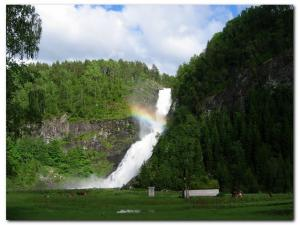
\includegraphics[scale=0.7]{huldefossen.jpg}
\end{frame}

\begin{frame}
\frametitle{The importance of water}
\begin{itemize}
\item 95 \% of domestic energy is supplied by hydropower.
\item A riparian system, waterfalls are privately owned.
\item Traditionally important to local communities.
\item By the 1830s, an estimated 20 000 - 30 000 watermills in operation.
\item Political and social ramifications.  
\item The emergence of a state monopoly in the early 20th century.
\end{itemize}
\end{frame}

\begin{frame}
\frametitle{Benefit sharing, historically}
\begin{itemize}
\item Market value, with a 25 \% premium.
\item Based on the market practices of the early 20th century.
\item The role of lay appraisers.
\item The push for a simple rule: the {\it natural horsepower method}.
\item Expropriation gaining ground.
\end{itemize}
\end{frame}

\begin{frame}
\begin{itemize}
\item From concrete assessment to theoretical assessment.
\item `Market' prices determined by looking to previous expropriation cases.
\item The lay appraisers are neutralised.
\item Only a symbolic form of benefit sharing?
\item The impossibility of deviating from the established formula.
\end{itemize}
\end{frame}

\begin{frame}
\frametitle{The effect of shaking up the regulatory system}
\begin{itemize}
\item Liberalization in the early 1990s.
\item Commercialization and (part) privatisation of the energy sector.
\item Local owners gain access to the distribution grid.
\item The real (commercial) value of water is revealed.
\item The case of Måren.
\end{itemize}
\begin{minipage}[t]{5cm}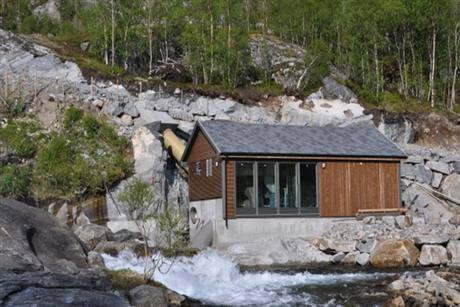
\includegraphics[scale=0.3]{smakraft.jpg}\end{minipage}
\begin{minipage}[t]{5cm}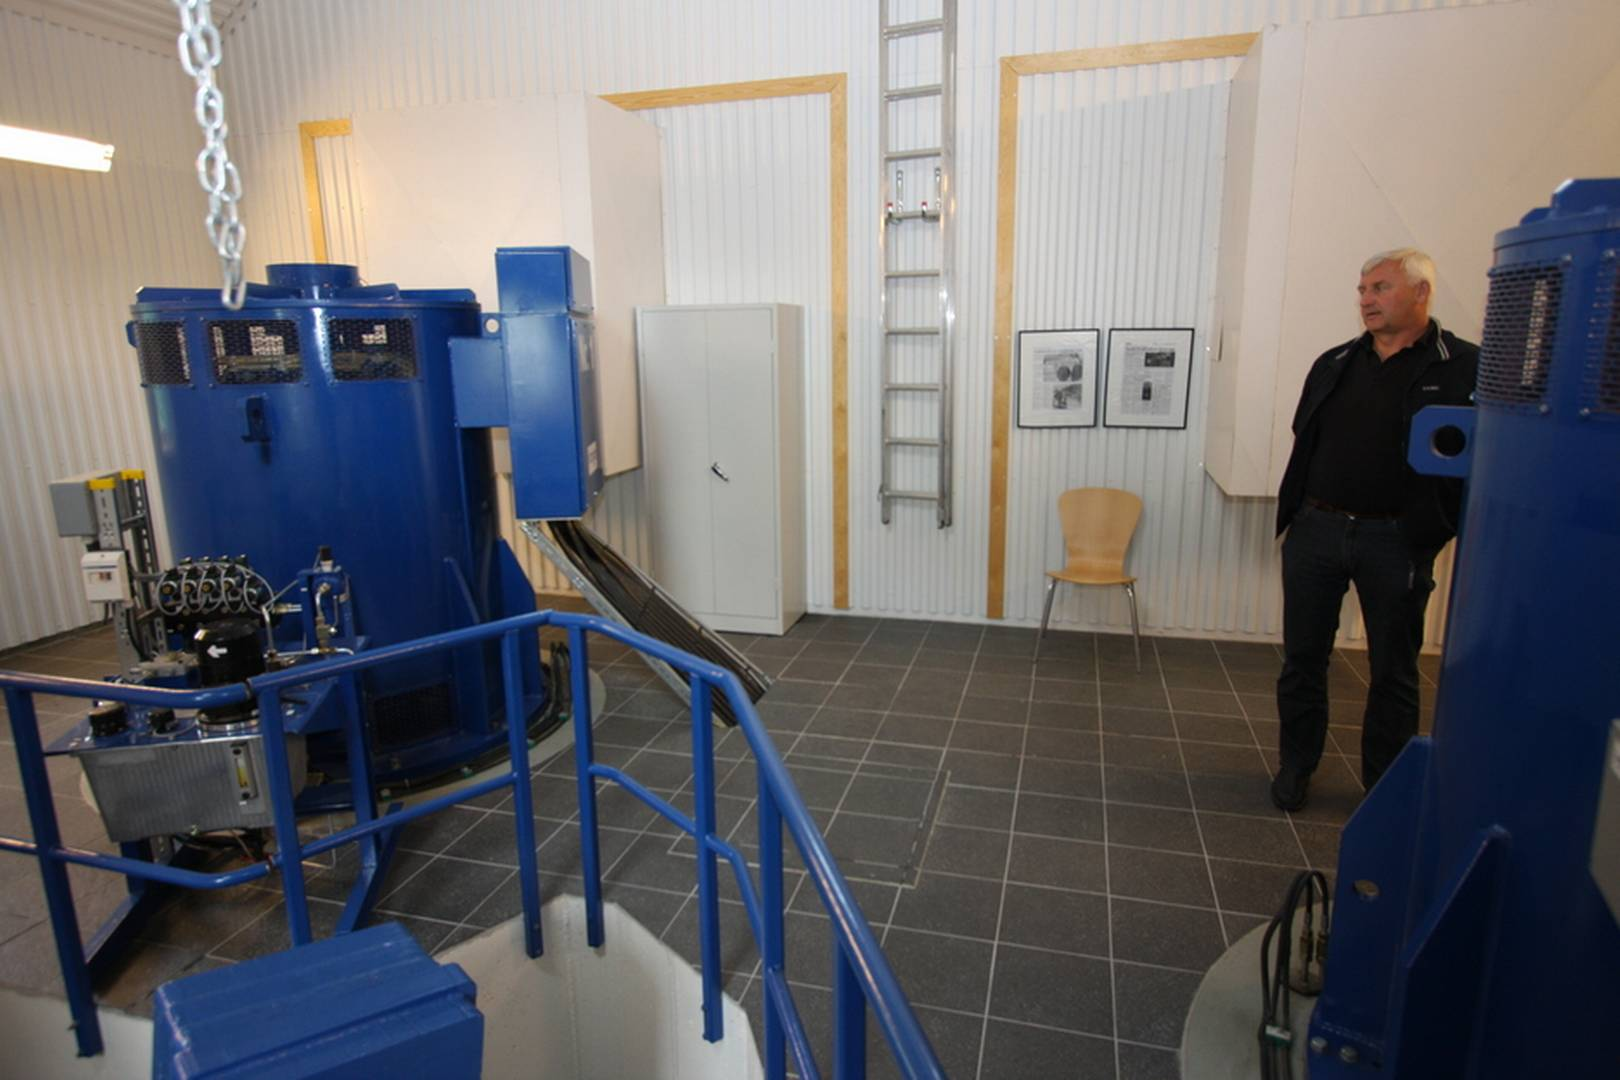
\includegraphics[scale=0.06]{smakraftt.jpg}\end{minipage}
\end{frame}

\begin{frame}
\frametitle{The effect of shaking up the regulatory system}
\begin{itemize}
\item Liberalization in the early 1990s.
\item Commercialization and (part) privatisation of the energy sector.
\item Local owners gain access to the distribution grid.
\item The real (commercial) value of water is revealed.
\end{itemize}
{\bf What about the compensation formula?}
\end{frame}

\begin{frame}
\frametitle{New principles for awarding compensation}
\begin{itemize}
\item No more natural horsepowers when alternative development is `foreseeable'.\footnote{Rt. 2008 s. 82.}
\item The {\it Pointe Gourde} principle is used to resist change: \pause
\begin{itemize}
\item On a narrow reading: The expropriation scheme belongs to the developer, not the owner.
\item On an average reading: The superiority of the resource-use of the expropriation scheme means that alternative development is not foreseeable.
\item On a broad reading: Other projects would be unprofitable or would not get planning permission.
\end{itemize}
\end{itemize}
\end{frame}

\begin{frame}
\frametitle{Uncertainty and a struggle for power}
\begin{itemize}
\item An extreme level of uncertainty. 
\item The importance of expert testimony (and having the resources to acquire it).
\item Diverging opinions in the Supreme Court.
\item {\it Kløvtveit}, Justice Bull:
\begin{quote}
None of the parties should be allowed to take a ``monopoly surplus'', either by inflating the price or, as far as the expropriating party is concerned, by arguing that they would have refused to cooperate in a joint development project, to make such a project unsuitable as the basis on which to calculate compensation.\footnote{Rt. 2011 s. 1683.}\end{quote} 
\end{itemize}
\end{frame}

\begin{frame}
\begin{itemize}
\item {\it Otra II}, Justice Matheson:
\begin{quote}
``[....] The Court of Appeal finds it difficult to distinguish this case from other cases when it has been established that alternative development is not foreseeable. It does not seem relevant whether this is the case because the alternative is not commercially viable or because the alternative must yield to a different exploitation of the waterfall''. I agree with the Court of Appeal...\footnote{Rt. 2013 s. 612}.\end{quote}
\end{itemize}
\end{frame}

\begin{frame}
\frametitle{The broader question}
\begin{itemize}
\item How should the hydropower sector be organized?
\item Who should benefit, who should decide?
\item What should be the role of expropriation?
\item Gloppen municipality, more than 250 GWh/year in owner-led projects.
\item The mayor: ``Small-scale hydropower is in our blood''.
\item When does benefit sharing become a human rights issue rather than a political issue?
\end{itemize}
\end{frame}

\section{Discussion}

\begin{frame}
\frametitle{Discussion}
\begin{itemize}
\item The problem of a narrative based on corrective justice.
\item The problem of a contextual narrative.
\item Drawing a distinction between `commercial' and `public' values.
\item Tracking the `pre-existent' commercial value.
\item Impossibility of fairness?
\item The importance of participation.
\item Alternatives to expropriation.
\end{itemize}
\end{frame}

\end{document}

\section{Conclusion}
\begin{frame}
\frametitle{Conclusion}
\begin{itemize}
\item
\end{itemize}
\end{frame}

\end{document}
%------------------------------------------------

\begin{frame}
\frametitle{Bullet Points}
\begin{itemize}
\item Lorem ipsum dolor sit amet, consectetur adipiscing elit
\item Aliquam blandit faucibus nisi, sit amet dapibus enim tempus eu
\item Nulla commodo, erat quis gravida posuere, elit lacus lobortis est, quis porttitor odio mauris at libero
\item Nam cursus est eget velit posuere pellentesque
\item Vestibulum faucibus velit a augue condimentum quis convallis nulla gravida
\end{itemize}
\end{frame}

%------------------------------------------------

\begin{frame}
\frametitle{Blocks of Highlighted Text}
\begin{block}{Block 1}
Lorem ipsum dolor sit amet, consectetur adipiscing elit. Integer lectus nisl, ultricies in feugiat rutrum, porttitor sit amet augue. Aliquam ut tortor mauris. Sed volutpat ante purus, quis accumsan dolor.
\end{block}

\begin{block}{Block 2}
Pellentesque sed tellus purus. Class aptent taciti sociosqu ad litora torquent per conubia nostra, per inceptos himenaeos. Vestibulum quis magna at risus dictum tempor eu vitae velit.
\end{block}

\begin{block}{Block 3}
Suspendisse tincidunt sagittis gravida. Curabitur condimentum, enim sed venenatis rutrum, ipsum neque consectetur orci, sed blandit justo nisi ac lacus.
\end{block}
\end{frame}

%------------------------------------------------

\begin{frame}
\frametitle{Multiple Columns}
\begin{columns}[c] % The "c" option specifies centered vertical alignment while the "t" option is used for top vertical alignment

\column{.45\textwidth} % Left column and width
\textbf{Heading}
\begin{enumerate}
\item Statement
\item Explanation
\item Example
\end{enumerate}

\column{.5\textwidth} % Right column and width
Lorem ipsum dolor sit amet, consectetur adipiscing elit. Integer lectus nisl, ultricies in feugiat rutrum, porttitor sit amet augue. Aliquam ut tortor mauris. Sed volutpat ante purus, quis accumsan dolor.

\end{columns}
\end{frame}

%------------------------------------------------
\section{Second Section}
%------------------------------------------------

\begin{frame}
\frametitle{Table}
\begin{table}
\begin{tabular}{l l l}
\toprule
\textbf{Treatments} & \textbf{Response 1} & \textbf{Response 2}\\
\midrule
Treatment 1 & 0.0003262 & 0.562 \\
Treatment 2 & 0.0015681 & 0.910 \\
Treatment 3 & 0.0009271 & 0.296 \\
\bottomrule
\end{tabular}
\caption{Table caption}
\end{table}
\end{frame}

%------------------------------------------------

\begin{frame}
\frametitle{Theorem}
\begin{theorem}[Mass--energy equivalence]
$E = mc^2$
\end{theorem}
\end{frame}

%------------------------------------------------

\begin{frame}[fragile] % Need to use the fragile option when verbatim is used in the slide
\frametitle{Verbatim}
\begin{example}[Theorem Slide Code]
\begin{verbatim}
\begin{frame}
\frametitle{Theorem}
\begin{theorem}[Mass--energy equivalence]
$E = mc^2$
\end{theorem}
\end{frame}\end{verbatim}
\end{example}
\end{frame}

%------------------------------------------------

\begin{frame}
\frametitle{Figure}
Uncomment the code on this slide to include your own image from the same directory as the template .TeX file.
%\begin{figure}
%\includegraphics[width=0.8\linewidth]{test}
%\end{figure}
\end{frame}

%------------------------------------------------

\begin{frame}[fragile] % Need to use the fragile option when verbatim is used in the slide
\frametitle{Citation}
An example of the \verb|\cite| command to cite within the presentation:\\~

This statement requires citation \cite{p1}.
\end{frame}

%------------------------------------------------

\begin{frame}
\frametitle{References}
\footnotesize{
\begin{thebibliography}{99} % Beamer does not support BibTeX so references must be inserted manually as below
\bibitem[Smith, 2012]{p1} John Smith (2012)
\newblock Title of the publication
\newblock \emph{Journal Name} 12(3), 45 -- 678.
\end{thebibliography}
}
\end{frame}

%------------------------------------------------

\begin{frame}
\Huge{\centerline{The End}}
\end{frame}

%----------------------------------------------------------------------------------------

\end{document} 